\section{Spectroscopy of the hyperfine structure}
\subsection{Set-up and procedure}
\begin{figure}[htb]
	\includegraphics[width=1.0\linewidth]{graphics/calibrationsetup}
	\caption[Experimental set-up for the Calibration]{Experimental set-up for the calibration measurements. An etalon is placed after the left lens and can be removed for the HFS-spectrum measurement.\cite{anleitung}}
	\label{fig:calibration setup}
\end{figure}
\subsubsection*{Laser scan-rate}
A Fabry-Pérot-Interferometer (etalon), which is a set of parallel, almost completely reflecting surfaces facing each other, is used to gauge the diode. The intensity at the photo diode will be drastically dampened unless the laser wavelength allows for constructive interference to occur between the surfaces. The wavelengths at which light passes the interferometer are thus equidistant.\\

The diode current is then modified with a saw-tooth voltage, which is also used to trigger the oscilloscope(see figure \ref{fig:calibration setup}). It is important to measure the scan-rate in a range of diode currents where the intensity response is linear and where the HFS-spectrum is actually visible (see next section). To get a solid calibration, at the very least 3 etalon peaks are necessary. These two factors have to be taken into consideration when choosing the measurement interval.\\ 

Figure \ref{fig:bendincurve} shows a bend in the diode current. Such areas need to be avoided when taking measurements, as they would lead to non-equidistant peaks in the etalon spectrum and unnecessarily complicate data analysis.
\begin{figure}
	\centering
	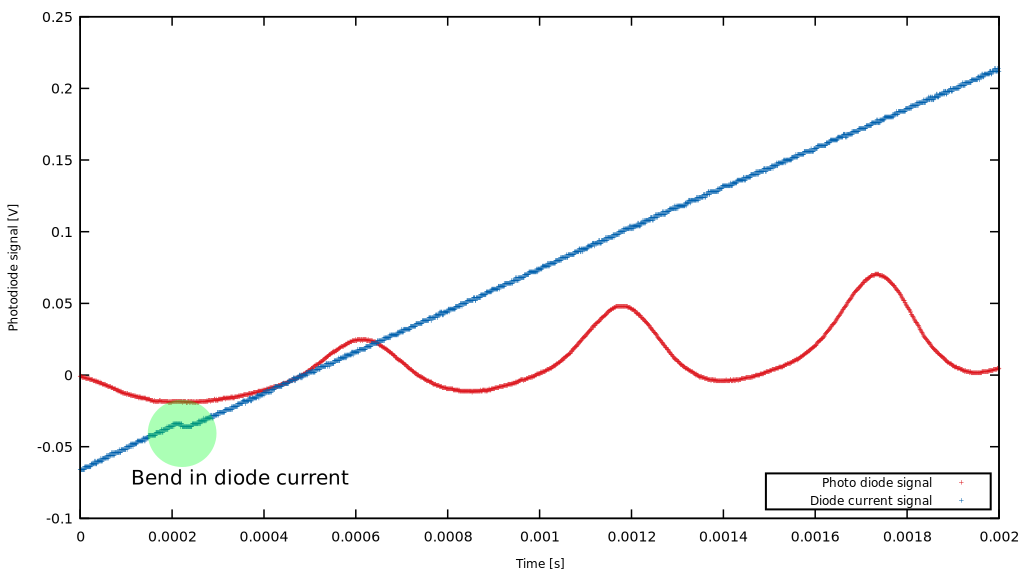
\includegraphics[width=1.0\linewidth]{graphics/bendincurve}
	\caption[Bend in modulating current]{In the bottom left corner, a clear bent in the diode current can be seen. These measurements were not used, a better current range was chosen instead.}
	\label{fig:bendincurve}
\end{figure}
The base current for the measurements was $I_L=\unit{(58.5\pm0.1)}{mA}$, where the uncertainty is the digit error of the multimeter ELTELEC, for which no data sheet was available. The temperature remained at $T=\unit{34.3}{\degree}$. The resulting intensity distribution can be seen in figure \ref{fig:etalon_fit}.

\subsubsection*{The HFS-spectrum}
The etalon is removed for this measurement and the exact same current modulation of the laser current as has been used for the scan-rate measurements will be used here as well. As the intensity increases with increasing diode current, the spectrum would have a linear offset. This can be counteracted by inverting the photo diode signal and adding the diode current signal to it. An additional cosmetic advantage of this is that the peaks are then positive.


\subsection{Data analysis}
\subsubsection*{Laser scan rate}
\begin{figure}[htb]
\centering
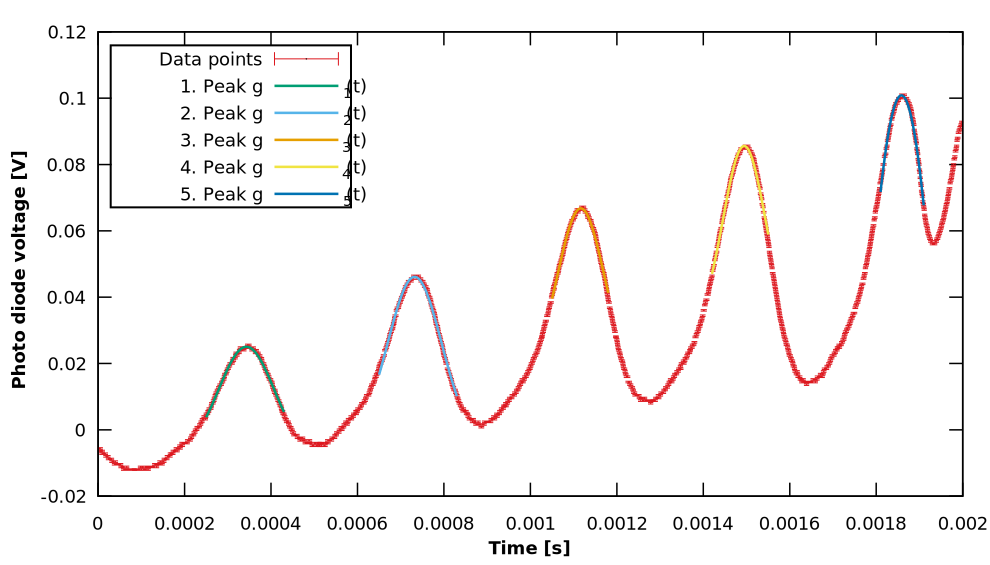
\includegraphics[width=1.0\linewidth]{graphics/etalon_fit}
\caption[Etalon peaks]{Results of the etalon calibration measurements. The rightmost peak is actually the same as the one on the left of it, as the saw-tooth reaches its peak between the two.}
\label{fig:etalon_fit}
\end{figure}
In figure \ref{fig:etalon_fit}, it has to be noted that the saw-tooth voltage reaches its maximum between the rightmost peak and the one on the left of it, meaning that these two actually belong to the same frequency. The rightmost peak is thus ignored for the calibration.\\
Gauss functions with a constant offset of the form
\begin{equation}
	g_i(t)=a_i*e^{-\frac{(t-t_{0,i})^2}{2*\sigma_i^2}}+c_i
	\label{eq:gaussfit}
\end{equation}
and a linear offset function $l(t)=b*t+c$ were used. 
The results for the peak positions $t_{0,i}$ can be seen in figure \ref{fig:ethalon_linearfit}. As the linear fit shows, these peaks are equidistant as expected with the time distance between peaks being $b=\unit{(0.379\pm0.003)}{ms}$. The nominal distance between two peaks is $\Delta_{FSR}=\unit{(9924\pm30)}{MHz}$. With these two values, the scan rate $r$ of the laser can be calculated as
\begin{equation}
	r=\unit{(26.17\pm 0.22)}{\frac{GHz}{ms}}
\end{equation}

\begin{figure}[htb]
\centering
\includegraphics[width=1.0\linewidth]{graphics/ethalon_linearfit}
\caption[Lienear fit on etalon peak positions]{Linear fit on the etalon peak positions.}
\label{fig:ethalon_linearfit}
\end{figure}

\subsubsection*{HFS-spectrum}
Only 6 of the expected 8 peaks (see fig. \ref{fig:hfslevels}) are visibly separated here. It is reasonable to assume that the peaks that were not separable are those of the transitions $^{85}$Rb F:3-2 and $^{85}$Rb F:3-3 as well as $^{85}$Rb F:2-2 and $^{85}$Rb F:2-3. This also means that the hyperfine constant for the $^2S_{\nicefrac{1}{2}}$ of $^{85}$Rb cannot be calculated with these measurements.
Gauss functions like those in equation \ref{eq:gaussfit} were used for the individual peaks. However, for the peaks that overlap, as sum of the two functions was used. For all fits, both a linear function and a constant were added and the total sum fitted to the data. The fit function for the last three peaks for example was
\begin{equation}
I_{4-6}(t)=g_4(t)+g_5(t)+g_6(t)+b\cdot t+c
\end{equation}
Table \ref{tb:HFSresults} lists the result of the fits as well as the frequency distances $\nu_{i}$ of the i-th peak to the first peak, which was arbitrarily chosen as a point of comparison. The differences between the peaks were compared to those expected (see fig. \ref{fig:hfslevels}) and the transitions were attributed accordingly. The uncertainties of the peak center times stem from the fits.\\

\begin{figure}[htb]
	\centering
	\includegraphics[width=1.0\linewidth]{graphics/HFS_fits}
	\caption[The HFS-spectrum]{The HFS-spectrum with fits to the individual peaks. The signal is negative since it was inverted.}
	\label{fig:HFS_fits}
\end{figure}


With these distances known and the help of equation \ref{eq:hfslevels}, the hyperfine constants can be calculated. For $A_{^2P_{\nicefrac{1}{2}}}(^{87}Rb)$, the calculation is
\begin{equation}
	A_{^2P_{\nicefrac{1}{2}}}(^{87}Rb)=h\cdot\frac{\nu_8-\nu_7}{F+1}=\unit{(1.52\pm0.18)}{\micro\electronvolt}
\end{equation}
where $F=1$ is the total angular momentum of the atom in the state that the transitions have in common. This value encloses the literature value $A_{^2P_{\nicefrac{1}{2}}}(^{87}Rb)=\unit{1.692}{\micro\electronvolt}$ \cite{corney} in its $1\sigma$ interval.\\
The other two calculable hyperfine constants are
\begin{align}
	A_{^2S_{\nicefrac{1}{2}}}(^{87}Rb)&=h\cdot\frac{\nu_8-\nu_2}{F+1}=\unit{(14.61\pm0.13)}{\micro\electronvolt}\\
	A_{^2S_{\nicefrac{1}{2}}}(^{85}Rb)&=h\cdot\frac{\nu_{5/6}-\nu_{3/4}}{F+1}=\unit{(4.50\pm0.08)}{\micro\electronvolt}
\end{align}
which both place their respective literature values $A_{^2S_{\nicefrac{1}{2}}}(^{87}Rb)=\unit{14.13}{\micro\electronvolt}$ and $A_{^2S_{\nicefrac{1}{2}}}(^{85}Rb)=\unit{4.185}{\micro\electronvolt}$ outside of their $3\sigma$ intervals. While the distance between the first and eigth peak of the spectrum is within $1\sigma$ of the expected value, the spectrum in between seems to be somewhat distorted. As we can also not separate the third and forth as well as the fifth and sixth peak, which are both more than 5 times further apart than the largest statistical error that was calculated, one has to assume that either the statistical errors are vastly underestimated or that there is a systematic error that is unaccounted for. Such a systematic error could be a not completely linear current modulation or the effect of the etalon not being placed perfectly perpendicular to the beam.

\begin{table}\centering
	\begin{tabular}{@{}llllllll@{}}
		\toprule
		&Peak $i$ &$t_0$ [ms]&$s_{t_0}$ $\unit{}{[\micro s]}$ &$\Delta\nu_{i}$ [GHz]&$s_{\Delta\nu_{i}}$ [GHz]&$\Delta\nu^{theo}_{i}$ [GHz]&Transition\\
		\midrule
		&1&0.104&0.18&-&-&-&$^{87}$Rb F:1-2\\
		&2&0.129&0.92&0.648&0.005&0.82&$^{87}$Rb F:1-1\\
		&3/4&0.215&0.05&2.905&0.024&2.66 / 3.02&$^{85}$Rb F:2-2/3\\
		&5/6&0.340&0.03&6.17&0.05&5.70 / 6.06&$^{85}$Rb F:3-2/3\\
		&7&0.371&0.06&6.98&0.06&6.83&$^{87}$Rb F:2-2\\
		&8&0.399&0.06&7.71&0.06&7.65&$^{87}$Rb F:2-1\\	
		\bottomrule
	\end{tabular}
	\caption[HFS peaks fit results]{Fit results of the Gauss fits on the HFS spectrum. The frequency calibration was used to calculate the frequency differences to the preceding peak. Theoretical values were taken from \cite{staatsex}.}
	\label{tb:HFSresults}
\end{table}
